% -*- mode: LaTeX; TeX-PDF-mode: t; -*- # Tell emacs file type (for syntax coloring)
% LaTeX path to the root directory of the current project, from the directory in which this file resides
% and path to econtexPaths which defines the rest of the paths like \FigDir
\providecommand{\econtexRoot}{}\renewcommand{\econtexRoot}{.}

\documentclass[\econtexRoot/Letter]{subfiles}
\onlyinsubfile{\externaldocument{\econtexRoot/Letter}} % Get xrefs -- esp to apndx -- from main file; only works if main file has already been compiled

\begin{document}
\notinsubfile{\renewcommand{\econtexRoot}{.}}

\hypertarget{job-market-paper}{}
%\par\section{Job Market Paper}
\notinsubfile{\label{sec:job-market-paper}}

%[Description of JMP and any other relevant work] \\

Will's job market paper (he will be on the 2024-25 market) is my favorite kind of exercise: Take some well-established microeconomic fact, incorporate it into a HANK macro model, and show that it has interesting macro implications that are not present until you match the micro reality. In Will's case, the micro fact is that exogenous spells of unemployment have a ``scarring effect'' on subsequent earnings. The micro literature has made the usual heroic efforts to establish that the measured scars are not due to some form of selection on unobservables - they are, as best one can tell, a causal consequence of an exogenous unemployment shock.  The simplest interpretation is that the spell results in a negative shock to idiosyncratic human capital.  (Other explanations, like a job ladder or match quality, would have the same consequences). Will embeds a micro structural model of unemployment into a general equilibrium setting, matches the facts on scarring, and explores the consequences in stagnating growth, raising income inequality, and reducing the effectiveness of fiscal austerity. In particular, he finds that unemployment scarring introduces a dimension that allows his model to capture both the sluggish growth in GDP following the Great Recession and the swift rebound in GDP from the COVID Recession. Furthermore, he demonstrates that scarring provides a rationale for why income inequality rose permanently following the Great Recession but only increased temporarily following the pandemic. He emphasizes that temporary layoffs complement fiscal policy in explaining the differences in recovery, and changes in income inequality, between the last two recessions. Specifically, Will demonstrates that the large fraction of temporary layoffs during the pandemic prevented a permanent decline in GDP and a permanent rise in income inequality. In the final exercise of his job market paper, he considers a counterfactual where the U.S. pursues fiscal austerity to reduce its debt-to-GDP. He finds that in the presence of scarring, austerity is four times less effective in reducing debt-to-GDP. 


%Will has made significant contributions to HARK, an open-source Python toolkit for solving heterogeneous agent models, with a focus on developing methods to compute heterogeneous agent Jacobians. These Jacobians are essential for solving general equilibrium models with rich microeconomic heterogeneity with the Sequence Space Jacobian methodology by \cite{Auclert2023}. Will has created several Jupyter notebooks illustrating how to use HARK to generate these Jacobians and solve general equilibrium HA models. Notably, he developed a notebook for simulating large heterogeneous agent economies with HARK (\href{https://github.com/econ-ark/HARK/blob/master/examples/ConsNewKeynesianModel/Transition_Matrix_Example.ipynb}{Simulation notebook}) and another for computing heterogeneous agent Jacobians (\href{https://github.com/econ-ark/HARK/blob/master/examples/ConsNewKeynesianModel/Jacobian_Example.ipynb}{Jacobian notebook}). He has also integrated his methods with the \href{https://github.com/shade-econ/sequence-jacobian}{Sequence Space Jacobian toolkit} to solve HANK models (\href{https://github.com/econ-ark/HARK/blob/master/examples/ConsNewKeynesianModel/SSJ_example.ipynb}{HANK notebook}) and a Krusell-Smith model without aggregate uncertainty (\href{https://github.com/econ-ark/HARK/blob/master/examples/ConsNewKeynesianModel/KS-HARK-presentation.ipynb}{Krusell-Smith Notebook}). For two consecutive years, Will has been invited to lecture on Sequence Space Jacobian methods in my Ph.D. computational economics course, for which he created a notebook explaining the mathematics and intuition behind the method (\href{https://github.com/econ-ark/HARK/blob/master/examples/ConsNewKeynesianModel/SSJ_explanation.ipynb}{notebook here}). During his tenure as a Ph.D. intern at the Bank of England, Will has leveraged his computational skills on solving general equilibrium models with rich microeconomic features to solve a HANK model with housing as a discrete choice (\href{https://github.com/wdu9/HANK_Housing_Block}{Slides and Code}). Heterogeneous agent models with discrete choice introduce a discrete continuous interaction that makes these models challenging to solve. An overview of the computational tools Will has developed can be found \href{https://www.william-du.com/computational-tools}{here}.




%Will has also made important contributions to HARK, an open source python toolkit for solving heterogeneous agent models. His contributions have largely focused on developing methods that compute heterogeneous agent Jacobians. These Jacobians are an essential object in solving general equilibrium models with rich microeconomic heterogeneity following the Sequence Space Jacobian methodology of \cite{Auclert2023}.  Will has produced several Jupyter notebooks demonstrating how to use the HARK code to produce these Jacobians and then solve general equilibrium models with rich micro heterogeneity. In particular, he has written notebooks on how to utilize his methods to simulate large heterogeneous agent economies with HARK (\href{https://github.com/econ-ark/HARK/blob/master/examples/ConsNewKeynesianModel/Transition_Matrix_Example.ipynb}{Simulation notebook}) and how to compute heterogeneous agent Jacobians (\href{https://github.com/econ-ark/HARK/blob/master/examples/ConsNewKeynesianModel/Jacobian_Example.ipynb}{Jacobian notebook}). In turn, Will has used the methods he constructed in these notebooks to write additional notebooks on how to combine HARK and the \href{https://github.com/shade-econ/sequence-jacobian}{Sequence Space Jacobian toolkit} to solve HANK models (\href{https://github.com/econ-ark/HARK/blob/master/examples/ConsNewKeynesianModel/SSJ_example.ipynb}{HANK notebook}) and a Krusell Smith model without aggregate uncertainty (\href{https://github.com/econ-ark/HARK/blob/master/examples/ConsNewKeynesianModel/KS-HARK-presentation.ipynb}{Krusell Smith Notebook}). For two consecutive years, I have invited Will to give a lecture on Sequence Space Jacobian methods in my Ph.D. computational economics course. For his lecture, Will created a jupyter notebook detailing the mathematics and intuition of the method (\href{https://github.com/econ-ark/HARK/blob/master/examples/ConsNewKeynesianModel/SSJ_explanation.ipynb}{notebook here}). 









%in a particular dimension: The consequences of a recession for subsequent output. To gauge the magnitude of the effects, Will does an exercise to evaluate the aftermath of the Great Recession in the United States and in the Euro zone, motivated by the fact that in Europe the byword for the fiscal response to the GR was ``austerity'' while in the US there was considerable stimulus (and a litany of criticism that the US should be pursuing austerity not stimulus). In Will's model, as in the data, the stimulative policy results in a much lower permanent drop in GDP than the austerity policy, corresponding to the actual outcomes in the US versus Europe.

%Consistent with the old literature suggesting that there is a unit root in GDP, Will finds that in his HANK model a recession results in a permanent reduction in the level of GDP because the shocks to human capital are permanent. These results connect not only with the old unit root and ``hysteresis'' literatures, but also with the newer ``secular stagnation'' literature. 





% Put here a link to the abstract of the JMP:

%%% Template for any figures
%\begin{figure}[ht!]
%	\centering
%	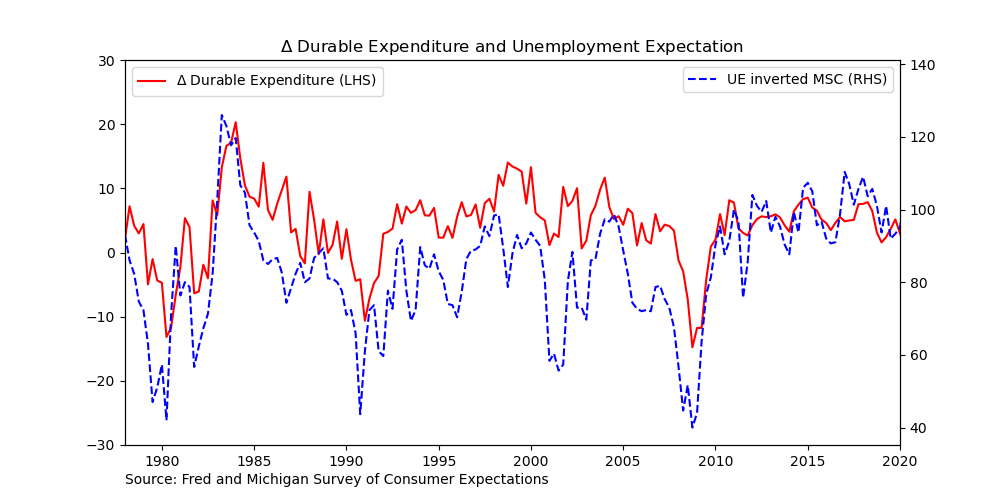
\includegraphics[width = 0.8\textwidth]{\FigDir/dur_vs_exp_emp.png}
	%\caption{Durable Expenditure and Expected Unemployment Rate} \label{fig:dur_vs_exp_emp}
%\end{figure}

\onlyinsubfile{% Allows two (optional) supplements to hard-wired \texname.bib bibfile:
% system.bib is a default bibfile that supplies anything missing elsewhere
% Add-Refs.bib is an override bibfile that supplants anything in \texfile.bib or system.bib
\provideboolean{AddRefsExists}
\provideboolean{systemExists}
\provideboolean{BothExist}
\provideboolean{NeitherExists}
\setboolean{BothExist}{true}
\setboolean{NeitherExists}{true}

\IfFileExists{\econtexRoot/Add-Refs.bib}{
  % then
  \typeout{References in Add-Refs.bib will take precedence over those elsewhere}
  \setboolean{AddRefsExists}{true}
  \setboolean{NeitherExists}{false} % Default is true
}{
  % else
  \setboolean{AddRefsExists}{false} % No added refs exist so defaults will be used
  \setboolean{BothExist}{false}     % Default is that Add-Refs and system.bib both exist
}

% Deal with case where system.bib is found by kpsewhich
\IfFileExists{/usr/local/texlive/texmf-local/bibtex/bib/system.bib}{
  % then
  \typeout{References in system.bib will be used for items not found elsewhere}
  \setboolean{systemExists}{true}
  \setboolean{NeitherExists}{false}
}{
  % else
  \typeout{Found no system database file}
  \setboolean{systemExists}{false}
  \setboolean{BothExist}{false}
}

\ifthenelse{\boolean{showPageHead}}{ %then
  \clearpairofpagestyles % No header for references pages
  }{} % No head has been set to clear

\ifthenelse{\boolean{BothExist}}{
  % then use both
  \typeout{bibliography{\econtexRoot/Add-Refs,\econtexRoot/\texname,system}}
  \bibliography{\econtexRoot/Add-Refs,\econtexRoot/\texname,system}
  % else both do not exist
}{ % maybe neither does?
  \ifthenelse{\boolean{NeitherExists}}{
    \typeout{bibliography{\texname}}
    \bibliography{\texname}}{
    % no -- at least one exists
    \ifthenelse{\boolean{AddRefsExists}}{
      \typeout{bibliography{\econtexRoot/Add-Refs,\econtexRoot/\texname}}
      \bibliography{\econtexRoot/Add-Refs,\econtexRoot/\texname}}{
      \typeout{bibliography{\econtexRoot/\texname,system}}
      \bibliography{        \econtexRoot/\texname,system}}
  } % end of picking the one that exists
} % end of testing whether neither exists
}

\ifthenelse{\boolean{Web}}{}{
  \onlyinsubfile{\captionsetup[figure]{list=no}}
  \onlyinsubfile{\captionsetup[table]{list=no}}
  \end{document}	\endinput
}

